\documentclass[utf8]{FrontiersinHarvard}
% for articles in journals using the Harvard Referencing Style (Author-Date), for Frontiers Reference Styles by Journal: https://zendesk.frontiersin.org/hc/en-us/articles/360017860337-Frontiers-Reference-Styles-by-Journal
%\documentclass[utf8]{FrontiersinVancouver} % for articles in journals using the Vancouver Reference Style (Numbered), for Frontiers Reference Styles by Journal: https://zendesk.frontiersin.org/hc/en-us/articles/360017860337-Frontiers-Reference-Styles-by-Journal

\usepackage{url,hyperref,lineno,microtype,subcaption}
\usepackage[T1]{fontenc}
\usepackage[english]{babel}
\usepackage{textcomp}
\usepackage{mdframed}
\usepackage{etoolbox} % For conditional statements
\usepackage{xstring}
\usepackage[normalem]{ulem} % todo: delete later
\usepackage{xparse}
\usepackage{makecell}
\usepackage{rotating}
\usepackage{pdfcomment}
\usepackage{xr}
\usepackage{cleveref}
\usepackage[nolist,nohyperlinks,printonlyused]{acronym}
\usepackage{wasysym} % for half bullet
\usepackage{pifont}
\usepackage{listings}
\usepackage{tcolorbox}



\definecolor{lightgray}{gray}{0.95} % Define light gray color
\definecolor{colorJan}{RGB}{18, 179, 77}
\definecolor{colorAthina}{RGB}{49, 133, 216}
\definecolor{colorEric}{RGB}{208, 83, 38}
\definecolor{colorWiktor}{RGB}{229, 209, 79}

\newcommand{\inlineBash}[1]{%
    \begingroup
    \edef\temp{#1}%
    \expandafter\StrSubstitute\expandafter{\temp}{--}{-{-}}[\temp]%
    \colorbox{lightgray}{\texttt{\small \temp}}%
    \endgroup
}

\newcommand{\inlinepy}[1]{\inlineBash{#1}}

%\newcommand{\inlineBash}[1]{\colorbox{lightgray}{\texttt{\small #1}}} % Command definition
%\newcommand{\inlineBash}[1]{\bold{#1}}

\newcommand{\missing}[1]{\textcolor{red}{\textbf{\MakeUppercase{#1}}}}

%\newcommand{\lbash}[1]{\lstset{frame=single} \begin{lstlisting}[language=bash] #1 \end{lstlisting}}

\newcommand{\fref}[1]{ (Figure~\ref{fig:#1})}

\newcommand{\todo}[3]{
% Define the default color
    \def\framecolor{orange}
    \def\framebgcolor{orange!20}
    \def\frametitlebgcolor{orange!40}

    % Check the person and assign the color
    \ifstrequal{#1}{Jan}{
        \def\framecolor{colorJan}
        \def\framebgcolor{colorJan!10}
        \def\frametitlebgcolor{colorJan!40}
    }{}
    \ifstrequal{#1}{Athina}{
        \def\framecolor{colorAthina}
        \def\framebgcolor{colorAthina!10}
        \def\frametitlebgcolor{colorAthina!40}
    }{}
    \ifstrequal{#1}{Eric}{
        \def\framecolor{colorEric}
        \def\framebgcolor{colorEric!10}
        \def\frametitlebgcolor{colorEric!40}
    }{}
    \ifstrequal{#1}{Wiktor}{
        \def\framecolor{colorWiktor}
        \def\framebgcolor{colorWiktor!10}
        \def\frametitlebgcolor{colorWiktor!40}
    }{}

    \begin{mdframed}[
        backgroundcolor=\framebgcolor,
        linewidth=1pt,
        linecolor=\framecolor,
        topline=true,
        bottomline=true,
        leftline=true,
        rightline=true,
        skipabove=\baselineskip,
        skipbelow=\baselineskip,
        frametitle={Todo @#1: #2},
        frametitlerule=true,
        frametitlebackgroundcolor=\frametitlebgcolor,
        frametitlerulewidth=1pt
    ]
        \centering
        #3
    \end{mdframed}
}

\externaldocument[supp-]{frontiers_SupplementaryMaterial}

\lstdefinestyle{bashStyle}{
    language=bash,
    frame=single,
    basicstyle=\footnotesize
}

\lstdefinestyle{pyStyle}{
    language=python,
    frame=single,
    basicstyle=\footnotesize
}

\lstdefinestyle{yaml}{
     basicstyle=\color{blue}\footnotesize,
     rulecolor=\color{black},
     string=[s]{'}{'},
     stringstyle=\color{blue},
     comment=[l]{:},
     commentstyle=\color{black},
     morecomment=[l]{-}
 }

% Define new commands for symbols to make the table cleaner
\newcommand{\cmark}{\ding{51}} % Check mark
\newcommand{\xmark}{\ding{55}} % Cross mark
\newcommand{\halfbullet}{\LEFTcircle} % Half bullet
\newcommand{\optional}{*} % Optional feature

\linenumbers

% Leave a blank line between paragraphs instead of using \\

\def\keyFont{\fontsize{8}{11}\helveticabold }
\def\firstAuthorLast{Reising {et~al.}} %use et al only if is more than 1 author
\def\Authors{Jan Philipp Reising\,$^{1,2}$, Ana Cristina Gonzalez-Sanchez\,$^{1,2}$, Athina Samara\,$^{1,2,3}$ and Eric
Herlenius\,$^{1,2*}$}
\def\Address{$^{1}$Department of Women's and Children's Health, Karolinksa Institutet, Stockholm, Sweden \\
    $^{2}$Astrid Lindgren Children’s Hospital, Karolinska University Hospital, Stockholm, Sweden \\
    $^{3}$Department of Biomaterials, FUTURE, Center for Functional Tissue Reconstruction, University of Oslo, Oslo,
    Norway
}

\def\corrAuthor{Eric Herlenius, CMM Center for Molecular Medicine L8:05, 171 76 Stockholm, Sweden}
\def\corrEmail{eric.herlenius@ki.se}

\begin{document}
    \onecolumn
    \firstpage{1}

    \title[Astrocytic Calcium Signaling Toolkit (astroCAST)]{Astrocytic Calcium Signaling Toolkit (astroCAST):
    Efficient Analysis of Dynamic Astrocytic Calcium Events }

    \author[\firstAuthorLast ]{\Authors} %This field will be automatically populated
    \address{} %This field will be automatically populated
    \correspondance{} %This field will be automatically populated

    % If there are more than 1 corresponding author, comment this line and uncomment the next one.
    \extraAuth{}

    %\extraAuth{corresponding Author2 \\ Laboratory X2, Institute X2, Department X2, Organization X2, Street X2, City X2, State XX2 (only USA, Canada and Australia), Zip Code2, X2 Country X2, email2@uni2.edu}

    \maketitle

    \begin{abstract}

        \section{}
        The \ac{astroCAST} is a novel solution to a longstanding challenge in neuroscience research: the specialized analysis of astrocytic calcium events within fluorescence time-series imaging. Distinguished from existing neuron-centric tools, \ac{astroCAST} is adept at detecting and clustering astrocytic calcium events based on their unique spatiotemporal characteristics, thus filling a gap in astrocytic research methodologies. This toolkit not only facilitates the detection of such events but also extends its utility to provide comprehensive end-to-end analysis, a feature absent in most astrocyte-focused tools. \ac{astroCAST}'s development was motivated by the critical need for dedicated software that supports researchers in transitioning from raw video data to insightful experimental conclusions, efficiently managing large-scale datasets without compromising computational speed. It offers a user-friendly interface that caters to both novice and expert users, incorporating both a \ac{GUI} for detailed explorations and a \ac{CLI} for handling extensive analyses. Expected outcomes from utilizing \ac{astroCAST} include the ability to process and analyze a significantly larger volume of data. This capability enables a more profound and comprehensive analysis than previously possible, addressing the demands of large-scale astrocytic studies. In summary, \ac{astroCAST} represents a significant step forward in astrocytic calcium imaging analysis, offering a tailored, efficient, and comprehensive toolset that enhances our understanding of astrocytic functions and their implications in neuroscience.

        \tiny
        \keyFont{ \section{Keywords:} astrocytes, toolkit, calcium, timeseries, detection, events} % 4 > tags < 9
    \end{abstract}

    \begin{acronym}
        \acro{1P}{One-photon}
        \acro{2P}{Two-photon}
        \acro{astroCAST}{Astrocytic Calcium Signaling Toolkit}
        \acro{CNN}{Convolutional Neural Network}
        \acro{preBötC}{pre-Bötzinger Complex}
        \acro{CLI}{command-line interface}
        \acro{GUI}{graphical user interface}
        \acro{FOV}{Field of View}
        \acro{RBF}{Radial Basis Function}
        \acro{RNN}{Recurring Neural Network}
    \end{acronym}

    \newpage

\section*{TODOs}

\todo{Jan}{Last checks}{
    \begin{itemize}
        \item Update figures
        \item \sout{check word count, manuscript length and figure number (\href{https://www.frontiersin.org/journals/cellular-neuroscience/for-authors/article-types}{Methods article or Technology and Code})}
        \begin{itemize}
            \item 12,000 words max (7169+160+879 -> 8208 words)
            \item 15 figures/tables total [currently 5 tables; 6 figures -> 11 total]
        \end{itemize}
        \item check supplementary material
        \item check all in-document references point to the correct section
    \end{itemize}
}

\todo{Ana}{Last checks}{
    \begin{itemize}
        \item Final read abstract, introduction, discussion
        \item \sout{Final read methods, results}
        \item Check name and affiliation
    \end{itemize}
}

\todo{Athina}{Last checks}{
    \begin{itemize}
        \item \sout{Final read abstract, introduction, discussion}
        \item Final read methods, results
        \item Check name and affiliation
    \end{itemize}
}

\todo{Eric}{Last checks}{
    \begin{itemize}
        \item Final read abstract, introduction
        \item Final read discussion and point out missing references
        \item Final read methods, results
        \item Final read Funding
    \end{itemize}
}

\newpage % todo: delete me later

    \section{Introduction}
    %! suppress = LineBreak

Astrocytes exhibit calcium fluctuations that are spatially and temporally diverse, reflecting their integration of a wide range of physiological signals\citep{semyanov_making_2020,smedler_frequency_2014}. Here, we provide a detailed guide for extracting these astrocytic calcium events from video recordings, performing clustering analysis, and correlating astrocyte activity with other physiological signals\fref{1}. This analysis has been applied to astrocytes in various settings, including acute slices, cell cultures, and in vivo recordings. Specifically, we demonstrate the application of astroCAST, using a custom dataset from a postnatal transgenic mouse brainstem, focusing on the \ac{preBötC}, as well as utilizing publicly available data.

\subsection{Requirements}
The initial step involves preparing the video recordings for analysis. Our protocol supports a range of file formats, including .avi, .h5, .tiff (either single or multipage), and .czi, accommodating videos with interleaved recording paradigms. To ensure reliable results, recordings should be captured at a frequency of at least 8Hz for \ac{1P} imaging and 1-2Hz for \ac{2P} imaging. This frequency selection is crucial for capturing events of the expected duration effectively. It is imperative that the recordings specifically capture astrocytes labeled with calcium sensors, either through transgenic models or viral vectors. While the use of calcium dyes is possible, their application may not guarantee the exclusive detection of astrocytic events.

Regarding hardware requirements, our protocol is adaptable to a variety of configurations, from personal computers to cloud infrastructures, with certain modules benefiting from GPU acceleration. At a minimum, we recommend using hardware equipped with a 1.6GHz quad-core processor and 16GB of RAM to efficiently handle the data analysis.

On the software side, we advocate for the use of Linux operating systems, specifically Ubuntu or AlmaLinux, for optimal performance, although Windows or macOS can be used with some functional limitations. Be advised, the M1 and M2 Mac processors are currently not supported, and we recommend using the docker image instead. However, even using the docker image it is not guaranteed that astroCAST will perform as expected. Essential software includes Python version 3.9, along with Anaconda or Miniconda for managing Python environments, and git for version control. An optional recommendation is ImageJ or an equivalent image viewer for analyzing the output visually. This comprehensive approach ensures that researchers can accurately extract and analyze astrocytic calcium signals, paving the way for further understanding of their physiological roles.


    \section{Methods}
    \todo{Athina}{Section name: 'Results' vs. 'Methods'}{I am not sure where to put the bulk of the previous protocol section. Should all the explanation of the toolkit steps go into the Methods or the Results. If it goes into the Results, what would go into the Methods?}



    \section{Results}
    \subsection{Installing \ac{astroCAST}}

\todo{Jan}{Functionality availability}{Table 1: Availability of different functionalities of astroCAST across
operating systems. A check mark () denotes full compatibility and active support. An asterisk () indicates that the
functionality is optional and can be installed upon user request (see below). A cross mark () signifies that the
functionality is not supported or available on the operating system. A half bullet () indicates partial support,
    indicating that the functionality is expected to be available but is not actively tested.  }

To run the software, you need to install the astroCAST package and its dependencies. There are multiple options to
install \ac{astroCAST} depending on how much control users would like to have over the installation. Of note, the
following instructions install astroCAST with its full functionality. If that is not desired or possible remove the \lstinline[style=bashStyle]{-E all} or \lstinline[style=bashStyle]{[all]} flags.

\subsubsection{Create conda environment}
While not strictly necessary, we highly recommend to create a fresh anaconda environment for the installation. This
prevents common installation errors and conflicts with existing environments.

\begin{lstlisting}[style=bashStyle]
    $ conda create -n astro python=3.9 poetry
    $ conda activate astro
\end{lstlisting}

\subsubsection{Install from source (recommended)}
\label{res:install-from-source}
\begin{lstlisting}[style=bashStyle]
    $ cd "/path/to/directory/"
    $ git clone git@github.com:janreising/astroCAST.git
    $ cd astroCAST
    $ poetry install –E all
\end{lstlisting}

\subsubsection{Installation with pip (easiest)}
\begin{lstlisting}[style=bashStyle]
    $ pip install astrocast[all]
\end{lstlisting}

\subsubsection{Container installation (last resort)}

To install docker and create an account, follow the instructions on the docker webpage: https://docs.docker
.com/engine/install/

\begin{lstlisting}[style=bashStyle]
    $ docker pull anacgon/astrocast:latest
    $ docker image ls
    $ docker run -v /path/to/your/data:/home/data -it -p 8888:8888 astrocast:latest
    # Optionally, start jupyter notebook from inside the docker container:
    $ jupyter-lab --allow-root --no-browser --port=8888 --ip="*"
\end{lstlisting}

\subsubsection{Test installation}

Both commands should run without any errors.

\begin{lstlisting}[style=bashStyle]
    $ python -c "import astrocast"
    $ astrocast --help
\end{lstlisting}

\subsection{Running astroCAST}

There are several ways to analyze data using \ac{astroCAST}, which we will reference throughout the protocol.

\subsubsection{Using jupyter notebooks}

Jupyter notebooks can be used to interactively run the analysis and visualize the results.
If you have cloned the repository (\ref{res:install-from-source}), an example notebook is included with the necessary
code to perform a basic analysis.

\begin{lstlisting}[style=bashStyle]
    $ cd "/path/to/astroCAST/notebooks/examples/"
    $ jupyter lab
    # on MacOS the command might be
    $ jupyter-notebook
\end{lstlisting}

A browser window will open which displays the available examples or can be used to create custom notebooks.

\subsubsection{Using the \ac{CLI}}
\todo{Jan}{CLI}{write exlanation for the client interface}

\subsubsection{Using the \ac{GUI}}
\todo{Jan}{GUI}{write exlanation for the GUI interface}

\subsection{Data showcase}

In this protocol, we demonstrate the utility of our toolkit using publicly available datasets and our own data.
The data represents astrocytes studied ex-vivo, in-vivo and in acute slices captured with One or Two Photon
microscopy recording speeds of 1-16Hz.

To ensure transparency and provide a practical starting point, we offer a collection of sensible, default settings
within a YAML file.
This file, designed to represent a first-approach configuration, is accessible in our GitHub repository.
Additionally, we provide the download of the datasets used here through a convenience function.
This repository serves as a comprehensive resource, aiding users in understanding and implementing the protocol with
similar data characteristics.

\todo{Jan}{1P and 2P acronyms}{}

Optionally, the available sample and training datasets can be directly downloaded from astrocast:
\begin{lstlisting}[style=bashStyle]
    $ astrocast download-datasets "/path/to/download/directory"
\end{lstlisting}

\todo{Jan}{pretrained models}{}

\begin{table}[ht]
    \centering
    \caption{Overview of Datasets Employed in Analysis}
    \begin{tabular}{|l|l|l|l|l|l|}
        \hline
        \textbf{Dataset}       & \textbf{Publication} & \textbf{Experiment}   & \textbf{Imaging Type} & \textbf{
            Imaging Speed} & \textbf{Number of files} \\ \hline
        custom:train/test      & unpublished          & acute slices, Gcamp6f & One-Photon            & 8 Hz
        & 49                       \\ \hline
        public: ExVivo         & AQuA                 & acute slices, Gcamp6f & Two-Photon            & 1.1 Hz
        & 1                        \\ \hline
        public: Glusnfr        & AQuA                 & acute slices, GluSnFR & Two-Photon            & 4-100 Hz
        & 1                        \\ \hline
        public: InVivo         & AQuA                 & in vivo GCamp6f       & Two-Photon            & 2 Hz
        & 1                        \\ \hline
        public: cellscan\_scim & CHIPS                & blood vessels, N/A    & Two-Photon            & N/A
        & 1                        \\ \hline
    \end{tabular}
\end{table}

\subsection{Pipeline approach}
The AstroCAST pipeline is structured into three major blocks: a) Preprocessing, b) Encoding and c) Exploratory Analysis.

In the Preprocessing block (a), users can navigate the pipeline through a \ac{CLI} by utilizing commands such as \lstinline[style=bashStyle]{$ astrocast --help}. This section allows for the utilization of a predefined configuration file to streamline the process. Additionally, an "Argument Explorer" is integrated to facilitate quick testing of various parameters and seamless export of the configuration file. If users want to follow this protocol along, we prepared a jupyter notebook for convenience.

During the Encoding (b) and Analysis (c) block, the approach varies based on the specificities of the experiment at
hand, be it comparing drug treatments, model systems, correlating with stimuli, or analyzing changes over time. This
segment of the pipeline now implements a separate GUI, offering a dynamic platform for detailed analysis and data
visualization.


    \subsection{Preprocessing}

\subsubsection{File conversion}
% Timing: 1-15 min (10M – 10Gpixels)
% Increasing the number of frames increases the processing time approximately linearly.

AstroCAST is designed to handle a wide range of common input formats, such as .tiff and .czi files, accommodating the diverse nature of imaging data in neuroscience research. One of the key features of astroCAST is its ability to process interleaved datasets. By specifying the \inlinepy{--channels} option, users can automatically split datasets based on imaging channels, which is particularly useful for experiments involving multiple channels interleaved, such as alternating wavelengths.

Moreover, astroCAST supports the subtraction of a static background from the video recordings using the \pyinline{--subtract-background} option. This feature allows for the provision of a background image or value, which is then subtracted from the entire video. Subtracting for example the dark noise of the camera can significantly enhance the quality of the analysis.

For optimal processing and data management, it is recommended to convert files to the .h5 file format. The .h5 format benefits from smart chunking, enhancing the efficiency of data retrieval and storage. The output configuration can be finely tuned with options such as \inlinepy{--h5-loc} for specifying the dataset location within the .h5 file, \inlinepy{--compression} for selecting a compression algorithm (e.g., `gzip`), and \inlinepy{--dtype} for adjusting the data type if the input differs from the intended storage format.

Chunking is a critical aspect of data management in astroCAST, allowing for the video to be divided into discrete
segments for individual saving and compression. The \inlinepy{--chunks} option enables users to define the chunk size, balancing between retrieval speed and storage efficiency. An appropriately sized chunk can significantly improve processing speed without compromising on efficiency. In cases where the optimal chunk size is uncertain, setting \inlinepy{--chunks} to \inlinepy{None} instructs astroCAST to automatically determine a suitable chunk size.

Lastly, the \inlinepy{--output-path} option directs astroCAST where to save the processed output. While the .h5 format is recommended for its efficiency, astroCAST also supports saving in formats such as .tiff, .tdb, and .avi, providing flexibility to accommodate various research needs and downstream analysis requirements.

\begin{lstlisting}[style=bashStyle]
    # (optional) browse the available flags
    $ astrocast convert-input --help
    # '--config' flag can be ommited to use default settings
    $ astrocast --config "/path/to/config" convert-input "/path/to/file/or/folder"
\end{lstlisting}

We recommend to verify the conversion through a quick visual inspection using the built-in data viewer\fref{2} or an imaging software of your choice (e.g., ImageJ). During this check, ensure that the pixel values are within the expected range (int or float), the image dimensions (width and height) are as anticipated, all frames have been successfully loaded, de-interleaving (if applicable) has been executed correctly, and the dataset name is accurate.

\begin{lstlisting}[style=bashStyle]
    $ astrocast view-data --h5-loc "dataset/name" "/path/to/your/output/file"
\end{lstlisting}

\todo{Jan}{add explanation for lazy parameter}{}

\subsubsection{Motion Correction (optional)}
% Timing: 1-15 min (10M – 10Gpixels)
% Increasing the number of frames increases the processing time approximately linearly.

During imaging, samples will drift or warp which means that the location of the astrocytes might change in the \ac{FOV}. Depending on the amount of movement, this can have detrimental consequences to the analysis. The motion correction module of the \href{https://github.com/flatironinstitute/CaImAn}{CaImAn} package\citep{giovannucci_caiman_2019}, is used in the astroCAST protocol to correct these artifacts. Please see \missing{Supplementary Video S1} for reference. We are including the commonly adjusted parameters here. We refer users to the the \href{https://jnormcorre.readthedocs.io/en/latest/Algo.html#motion-correction-methods}{jnormcorre documentation} for detailed information.

A cornerstone of this feature is the ability to set the maximum allowed rigid shift through the \inlinepy{--max-shifts} parameter. This parameter is critical for accommodating sample motion, ensuring that shifts do not exceed half of the image dimensions, thus balancing between correction effectiveness and computational efficiency. The precision of motion correction is further refined using the \inlinepy{--max-deviation-rigid} option, which limits the deviation of each image patch from the frame's overall rigid shift. This ensures uniformity across the corrected image, enhancing the fidelity of the motion correction process. For iterative refinement of the motion correction, astroCAST employs the \inlinepy{--niter-rig} parameter, allowing up to three iterations by default. This iterative approach enables a more accurate adjustment to the motion correction algorithm, improving the quality of the processed images. To address non-uniform motion across the field of view, astroCAST offers the piecewise-rigid motion correction option, activated by setting \inlinepy{--pw-rigid} to True. This method provides a more nuanced correction by considering different motion patterns within different image segments, leading to superior correction outcomes. Furthermore, the \inlinepy{--gsig-filt} parameter anticipates the half-size of cells in pixels. This information aids in the filtering process, crucial for identifying and correcting motion artifacts accurately.

By carefully adjusting these parameters, researchers can significantly enhance the quality of their imaging data, ensuring that motion artifacts are minimized and that the resultant data is of the highest possible fidelity for subsequent analysis.

\begin{lstlisting}[style=bashStyle]
    # '--config' flag can be ommited to use default settings
    $ astrocast --config "/path/to/config" motion-correction --h5-loc "dataset/name" "/path/to/file"
\end{lstlisting}

\subsubsection{Denoising (optional)}
% Timing: 1-12 h (first time), 1-30 min (inference)

Denoising is an optional but often beneficial preprocessing step in image analysis. The denoising module is based on the architecture suggested in the DeepInterpolation publication\citep{lecoq_removing_2021} and employs a \ac{CNN} designed to clean a target frame.The \ac{CNN} uses adjacent frames as a reference without exposing it to the target frame itself. This approach enables the network to interpolate the desired signal from the contextual frames. Since the noise is stochastic, the network inherently learns to disregard it, effectively isolating and enhancing the signal in the process. We have extended the original approach to support videos of varying dimensions and facilitate straightforward retraining protocols.

Training the denoising model is typically a singular task; once the model is trained, it can be applied to multiple datasets with no further adjustments. The duration of this initial training varies from 1 to 12 hours, contingent on data intricacy and available computational power. Subsequent application of the model to new data, known as inference, is considerably more expedient, usually requiring minutes for each file.

For convenience, we offer a suite of pretrained models tailored to different imaging modalities. A curated list is accessible on our GitHub page under \href{https://github.com/janreising/astroCAST/tree/main/denoiser_models}{denoiser models}, and a comprehensive collection of models can be downloaded via \ac{astroCAST].

\begin{lstlisting}[style=bashStyle]
    $ astrocast download-models "/path/to/download/directory/"
\end{lstlisting}

\todo{Jan}{model naming convention}{Explain the naming convention for the model files.}

\paragraph{Training (optional)}

To ensure the robustness and reliability of the denoising process, it is crucial to carefully select the training dataset for the denoiser model. The approach to training should aim to minimize the model's exposure to the data it will denoise, which can enhance the reliability of denoising and prevent overfitting.

One approach is to train the model on a separate data set that will not be used in subsequent analysis. This method is advantageous because it allows the model to learn from a diverse set of data, ideally encompassing all experimental conditions expected in the study. However, it requires having a separate dataset that is representative of the various modalities, which may not always be available.

For smaller datasets or when data is limited, a transformation-based approach can be applied. Training on all experimental data but using rotated frames (90°, 180°, and 270°) ensures that the denoiser is exposed to the inherent noise and variability in the data while mitigating direct exposure to the frames being denoised. This approach is particularly resource-efficient but may result in a less robust model due to the potential predictability of rotated frames.

Each of these methods has its merits and should be chosen based on the specific context and availability of data within a given study.

\begin{lstlisting}[style=bashStyle]
    # explore the possible parameters
    $ astrocast train-denoiser --help
    # train model from config file
    $ astrocast --config config.yaml train-denoiser
\end{lstlisting}

The intricacies of training a custom model are beyond this protocol, and we refer to the original DeepInterpolation
publication\citep{lecoq_removing_2021} and our \href{https://github.com/janreising/astroCAST/blob/8451394bc0d810c4037011f0bcb9cba1f10d1e72/notebooks/examples/train_denoiser_models.ipynb}{example notebook} for users interested in training their own model.

\todo{Jan}{Better notebook}{Maybe it makes sense to write a better tutorial.}

\paragraph{Denoising Data}
Once the neural network has been trained for denoising, it can be employed on new data using the parameters that were set during its training\fref{3}. If utilizing a provided pretrained model, these parameters are inferred from the model file.

For trivial input parameters, such as the model path and output file location, the following flags are used: \inlinepy{--model} to specify the model, \inlinepy{--output-file} to define the output file, \inlinepy{--loc-in} and \inlinepy{--loc-out} to designate the input and output data locations within the HDF5 file structure.

Network architecture parameters are crucial for ensuring that the denoising process is compatible with the data's specific attributes. These parameters need to exactly match the parameters during training. These include \inlinpy{--input-size} to set the dimensions of the input data, \inlinepy{--pre-post-frames} to determine the number of frames before and after the target frame used during denoising, \inlinepy{--gap-frames} to optionally skip frames close to the target frame, and \inlinepy{--normalize} to apply normalization techniques that aid the network in emphasizing important features over noise.

Image parameters cater to the post-processing needs of the denoised data. The \inlinepy{--rescale} parameter is used to reverse the normalization applied during denoising, as subsequent analysis steps often expect the pixel values to be in their original scale. Furthermore, \inlinepy{--padding} adjusts the input data size to match the network's expected input dimensions, ensuring that no data is lost or distorted during the denoising process.

\begin{lstlisting}[style=bashStyle]
    # load a config file with parameters
    $ astrocast --config config.yaml denoise "/path/to/file"
\end{lstlisting}

%%%%%%%%%%%%%%%%%%%%%%%%%
%% Background subtraction

\subsubsection{Background subtraction (optional)}
\label{subsubsec:background}
% Timing: 1-20 min
% Running time will increase linearly with the number of frames and non-linearly with window size.

Background subtraction, while optional, can significantly enhance event detection in fluorescence imaging by mitigating issues related to bright backgrounds, uneven lighting, or pronounced bleaching effects\fref{4}. AstroCAST leverages \ac{RBF} interpolation for background approximation, ensuring accurate background modeling even in scenarios characterized by considerable signal fluctuations or missing data segments.

To facilitate optimal subtraction outcomes without introducing artifacts such as false positives or negatives, default parameters are provided, but fine-tuning may be necessary. An exploratory Jupyter \href{https://github.com/janreising/astroCAST/blob/8451394bc0d810c4037011f0bcb9cba1f10d1e72/notebooks/dev/exploring_delta.ipynb}{notebook} is available for guidance on how parameter adjustments influences the results.

% Intuition behind the process
The process begins with downsizing the video to manage computational load while preserving essential features. Peaks within each pixel's time series are identified and marked as NaN to exclude them from influencing the background model. The RBFInterpolator then estimates the background by interpolating these NaN values across the XYZ dimensions of the video, which is subsequently resized to its original dimensions, and the interpolated background is subtracted.

% Image preparation parameters
For initial image preparation, parameters such as \inlinepy{--scale-factor} for adjusting video resolution, \inlinepy{--blur-sigma} and \inlinepy{--blur-radius} for image blurring, are crucial. These adjustments are preparatory steps aimed at enhancing the effectiveness of the subsequent background subtraction process.

% Peak detection parameters
Peak detection is fine-tuned through parameters like \inlinepy{--prominence}, \inlinepy{--wlen} for window length, \inlinepy{--distance} between peaks, \inlinepy{--width} of peaks, and \inlinepy{--rel-height} defining the peak's cutoff height. These settings ensure precise identification of significant peaks, contributing to the accuracy of the background modeling.

% RBF parameters explanation
The \href{https://docs.scipy.org/doc/scipy/reference/generated/scipy.interpolate.RBFInterpolator.html}{RBF interpolator} constructs a smooth function from scattered data points by combining radial basis functions centered at data locations with a polynomial term, adjusted by coefficients that solve linear equations to fit the data. Interpolation can be tunes with parameters such as \inlinepy{--neighbors} for the interpolation neighborhood, \inlinepy{--rbf-smoothing} for interpolation smoothness, \inlinepy{--rbf-kernel} to choose the kernel type, \inlinepy{--rbf-epsilon}, and \inlinepy{--rbf-degree} for kernel adjustment, facilitating a tailored approach to background modeling.

% Method selection for background subtraction
Background subtraction can be executed using either the Delta F (\inlinepy{--method} `dF`) method, which directly subtracts the background, or the Delta F over F (\inlinepy{--method} `dFF`) method, which divides the signal by the background post-subtraction. The choice between these methods depends on the specific requirements of the imaging data and the desired outcome of the subtraction process. However, it's important to consider that background subtraction may not be necessary for all datasets and could potentially introduce biases in event detection. Comparative analysis with and without this preprocessing step is recommended to assess its impact accurately.

\begin{lstlisting}[style=bashStyle]
    $ astrocast subtract-background --h5-loc "mc/ch0" --method "dF" "/path/to/file"
\end{lstlisting}
\subsection{Event Detection}
%Timing: 1 min – 3h
%Running time will increase linearly with the number of events in the recording. 

AstroCAST employs an event-centric approach to event detection, adapted from the AQuA package\citep{wang_event-based_2018}. Building on the AquA algorithm, astroCAST incorporates both spatial and temporal thresholding
techniques to identify and extract events effectively. Spatial thresholding is executed based on either a single
frame or a small volume, facilitating the identification of significant patterns or features in space. Concurrently,
temporal thresholding is implemented by scrutinizing individual pixels for peaks across the time dimension,
essentially tracking fluorescence changes over time.

Following the thresholding process, a binary mask is generated, which is used to label connected pixels, considering
the full 3D volume of the video. This allows for the integration of different frames in the z-dimension to constitute
a single event in a 3D context, ensuring a comprehensive analysis of the events captured in the video. Upon
successful event detection, our protocol generates a folder with a .roi extension. This folder houses all files
related to the detected events, offering an organized and accessible repository for the extracted data.

The event detection step is the most critical aspect of astroCAST and is sensitive to the choice of parameters. We
have therefore implemented an interactive interface to explore the performance of each step during event detection
given the relevant options. The program will prompt a link to the browser-based interface. We recommend to select a
short range of frames in the video file to keep processing time during exploration short.

\begin{lstlisting}[style=bashStyle]
    $ astrocast explorer -- input path "/path/to/file" -- h5-loc "/dataset/name"
\end{lstlisting}

Once users are satisfied with the chosen parameters, they can be exported to a YAML config file, that can be provided
to the astrocast \ac{CLI}.

\subsubsection{Detection Module Description}
The detection module in AstroCAST applies a comprehensive approach to identify astrocytic events by smoothing,
thresholding, and applying morphological operations on fluorescence imaging data. This section outlines the key steps
and parameters used in the process.

\paragraph{Smoothing}
AstroCAST incorporates a Gaussian smoothing kernel to enhance event detection while preserving spatial features.
Adjusting the \lstinline[style=bashStyle]{--sigma} and \lstinline[style=bashStyle]{--radius} parameters allows for
the refinement of the smoothing effect, ensuring that events are emphasized without compromising the integrity of
spatial characteristics. The smoothed data then serve as the basis for subsequent detection steps, although users can
opt out of smoothing if desired.

\paragraph{Thresholding}
\todo{Jan}{Active pixels}{thresholding -> identifying active pixels}
Thresholding in AstroCAST is executed in two phases, spatial and temporal, to classify pixels as active with high
precision.

Spatial thresholding evaluates the entire frame to distinguish active pixels, automatically determining a cutoff
value. It incorporates the mean fluorescence ratio of active to inactive pixels to mitigate the misidentification of
noise as events. The \lstinline[style=bashStyle]{--min-ratio} parameter sets the minimum ratio threshold, and the \lstinline[style=bashStyle]{--z-depth} parameter allows for the consideration of multiple frames to improve threshold accuracy.

Temporal thresholding analyzes the video as a series of 1D time series, identifying peaks with a prominence above a
user-defined threshold. Parameters such as \lstinline[style=bashStyle]{--prominence}, \lstinline[style=bashStyle]{--width}
, \lstinline[style=bashStyle]{--rel-height}, and \lstinline[style=bashStyle]{--wlen} fine-tune the detection of
events over time, enhancing the separation of true events from noise.

Combining spatial and temporal thresholding, users can choose to merge or differentiate the active pixels identified
by each method, optimizing event detection based on specific dataset characteristics.

\paragraph{Morphological Operations}
To address artifacts resulting from thresholding, such as holes (false negatives) and noise (false positives),
AstroCAST employs morphological operations. Parameters like \lstinline[style=bashStyle]{--area-threshold} and \lstinline[style=bashStyle]{--min-size} adjust the maximum hole size to fill and the minimum size of active pixel clusters, respectively. These operations, which also consider connectivity and the \lstinline[style=bashStyle]{--z-depth} parameter, refine the detection outcome by smoothing gaps and removing minor artifacts, enhancing the clarity and segmentation of detected events.

\paragraph{Additional options}
Additionally, AstroCAST provides the option to exclude the video border from active pixel detection (\lstinline[style=bashStyle]{--exclude-border}) to mitigate motion correction artifacts. An experimental feature (\lstinline[style=bashStyle]{--split-events}) is available for separating incorrectly connected events, further improving the accuracy of event detection.

\todo{Jan}{Figure}{Add figure combining several previous figures: overview???; Fig. 8 (temporal thresholding; Spatial
thresholding??; Fig. 12: Detected events overlay )}

\subsubsection{Evaluating Detection Quality}
AstroCAST offers a streamlined approach for assessing the quality of event detection through its command-line interface.

\begin{lstlisting}[style=bashStyle]
    $ astrocast view-detection-results "/path/to/roi"
\end{lstlisting}

Researchers can visually inspect the detection outcomes. During this evaluation phase, it is crucial to determine whether the detection process has successfully identified all expected events, thereby minimizing false negatives, and to assess the correctness of these events to ensure that noise has not been misclassified as true events, which would indicate false positives. If the detection results are not satisfactory, revising the event detection parameters or adjusting settings in the preceding background subtraction step (\ref{subsubsec:background})may be necessary to achieve improved accuracy. For a dynamic visualization that illustrates the impact of parameter adjustments on detection outcomes, researchers are directed to consult \missing{Supplementary Video S2}.

\todo{Jan}{not entirely true}{The video is more about expected results.}

\subsection{Clustering}


    \section{Discussion}
    \subsection{Expected outcomes}

\todo{Athina}{Include input from Jan}{
Actual Limitations:
\begin{itemize}
    \item Lack of a fully developed Astrocyte Simulator for toolkit testing. Additionally, could be used to detect events through iterative simulation refinement. Basically building a virtual copy of the cell population imaged.
    \item Suboptimal GUI responsiveness, limited by my front-end development skills.
    \item Incomplete implementation of "inference-of-cell" for assigning events to individual cells. The "Functional Units" module exists as an experimental feature but lacks proper validation and testing due to time constraints and insufficient biological data (e.g., sparse Gcampf6 expression recordings or post-imaging staining).
\end{itemize}

Intended Audience:
\begin{itemize}
    \item Bioinformaticians or neuroscientists with a programming background.
    \item necessary: expertise in Python and running command line tools; troubleshooting code
    \item optional: experience in image analysis, time series clustering, machine learning
\end{itemize}

Additional Notes:
\begin{itemize}
    \item Consider making titles more complex to accurately reflect the content's sophistication.
    \item Highlight the need for interdisciplinary analysis in neuroscience, particularly for astrocyte datasets, emphasizing the collaborative effort required.
\end{itemize}
}

AstroCAST could facilitate several key outcomes for researchers working with astrocytic calcium imaging data analysis
. On the technical front, the tool is designed to handle large-scale datasets effectively. For example, in time
-lapse recordings of astrocytes at 20X magnification and 1024x1024 pixel resolution, astroCAST is equipped to
identify up to 1,000 astrocytic events per 100 frames. As the analysis progresses, users should find that the
software can comfortably manage up to 50,000 events using the encoding algorithms provided. This performance equates
to the comparative analysis of around 15 time-lapse videos, each with a 20-minute recording time. Furthermore,
astroCAST is designed to efficiently handle larger datasets, efficiently analyzing more events than previously
possible in astrocyte-specific studies. This is achieved without compromising on computational time. From an
innovation standpoint, astroCAST offers more than just event detection. Users can expect a cohesive, end-to-end
analytical workflow that guides them from raw video data to insightful experimental conclusions. The software brings
structure and flexibility to the often-challenging variable-length timeseries analysis, setting it apart as a unique
tool in the field of astrocytic calcium imaging.

\subsection{Limitations}

The astroCAST protocol has proved to be effective in analyzing calcium events in fluorescence imaging data. We have
tested the system in depth on acute slices, as well as available public data for in-vivo and cell culture recordings
. There are, however, challenges that might be considered as limitations. For example, astroCAST can firmly attribute
events to individual cells, but is agnostic to cell shape by design, enabling us to analyze recordings even when
cells overlap or change morphology. Furthermore, issues that stem from the difficulty to distinguish close bordering
events, the computational complexity, the event length and data dimensionality, and others, may also need fine-tuning
. We acknowledge that users might encounter some of these, and we make suggestions for each in the troubleshooting
section.

We consider the fact that astroCAST is user customizable to be an asset that will aid researchers globally to
decipher the enigmatic astrocytic calcium activity.

    \section*{Conflict of Interest Statement}
    The authors declare that the research was conducted in the absence of any commercial or financial relationships that could be construed as a potential conflict of interest.

    \section*{Author Contributions}
    JPR and EH conceptualized the study and EH secured funding for the project. JPR designed the algorithms, conducted the data analysis, and contributed to the building of the astroCAST toolkit. ACGS collaborated with JPR in building the toolkit. JPR wrote the manuscript, with contributions from ACGS and AS. EH and AS provided supervision throughout the project. All authors reviewed and approved the final manuscript.

    \section*{Use of Generative AI}
    During the preparation of this manuscript, we utilized the generative capabilities of OpenAI's ChatGPT-4. The AI's primary role was to assist in proofreading and language refinement to ensure clarity, conciseness, and readability of the text. While the AI provided suggestions for language adjustments, the final manuscript content was thoroughly reviewed, curated, and approved by the authors. We, the authors, take full and complete responsibility for the integrity and accuracy of the manuscript content.

    \section*{Funding}
    This study was supported by grants to EH from the Swedish Research Council (2019–01157), the Stockholm County Council (2019–0400, 2019–0974 and FoUI-966 449), the Swedish Brain (FO2019-0087 and FO2021-0313), the Swedish National Heart and Lung (2018 0505 and 2021 0579), the Axel Tielmans, the Freemasons Children's House foundations and Karolinska Institutet. The funders did not participate in the design or conduct of the study.

    \todo{Eric}{Check funding}{Eric, could you have a look at this section.}

    \section*{Acknowledgments}
    \todo{Jan}{Acknowledgments}{
        \begin{itemize}
            \item Animal facility and Staff (KMB)
            \item The development of this toolkit was enabled by resources in projects SNIC 2022/22-1224 and SNIC 2022/23-638 provided by the National Academic Infrastructure for Supercomputing in Sweden (NAISS) at UPPMAX, funded by the Swedish Research Council through grant agreement no. 2022-06715.
        \end{itemize}
    }

    \section*{Supplemental Data}
    \href{http://home.frontiersin.org/about/author-guidelines#SupplementaryMaterial}{Supplementary Material} should
    be uploaded separately on submission, if there are Supplementary Figures, please include the caption in the same
    file as the figure. LaTeX Supplementary Material templates can be found in the Frontiers LaTeX folder.

    \section*{Data Availability Statement}
    Further information and requests for resources and reagents should be directed to and will be fulfilled by the lead contact, Eric Herlenius [eric.herlenius@ki.se]. All original code has been deposited at \href{https://github.com/janreising/astroCAST}{astroCAST}.

    \bibliographystyle{Frontiers-Harvard} %  Many Frontiers journals use the Harvard referencing system (Author-date), to find the style and resources for the journal you are submitting to: https://zendesk.frontiersin.org/hc/en-us/articles/360017860337-Frontiers-Reference-Styles-by-Journal. For Humanities and Social Sciences articles please include page numbers in the in-text citations
    %\bibliographystyle{Frontiers-Vancouver} % Many Frontiers journals use the numbered referencing system, to find the style and resources for the journal you are submitting to: https://zendesk.frontiersin.org/hc/en-us/articles/360017860337-Frontiers-Reference-Styles-by-Journal
    \bibliography{astrocast}

    \section*{Figure captions}
    \begin{figure}[h!]
\begin{center}
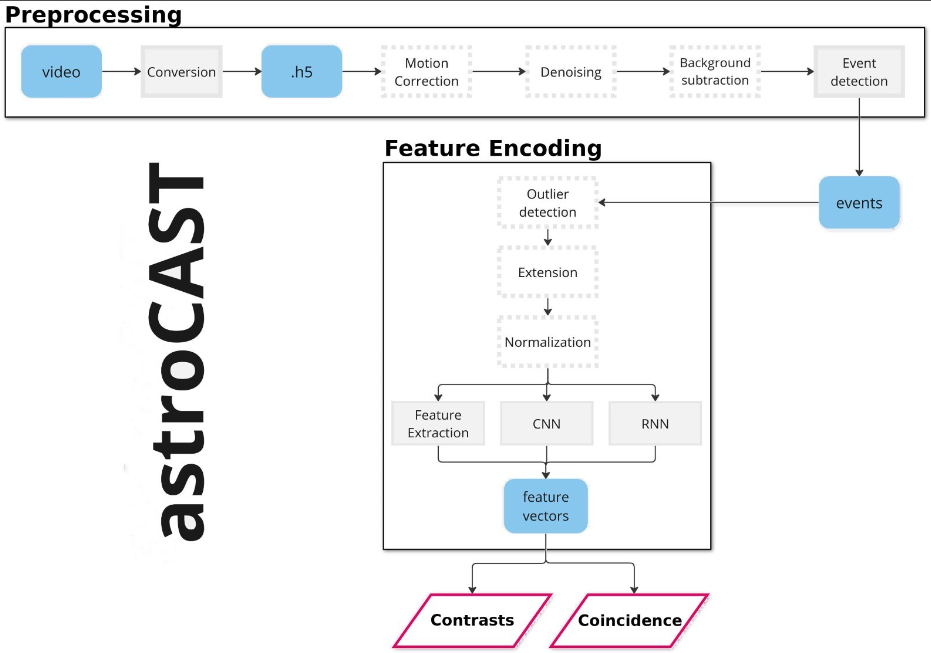
\includegraphics[width=\linewidth]{figures/1.png}
\end{center}
\caption{AstroCAST Pipeline Overview: First box shows how the input video is converted and processed to detect events. Second box shows how the detected events undergo feature extraction utilizing different approaches to generate feature vectors. Last steps shows how feature vectors can be analyzed to identify patterns and correlations. Optional steps in the pipeline are indicated by dotted boxes, and outputs at each stage are shown in blue. Exemplary types of experiments explained in this protocol are highlighted in red.}\label{fig:1}
\end{figure}

\begin{figure}[h!]
\begin{center}
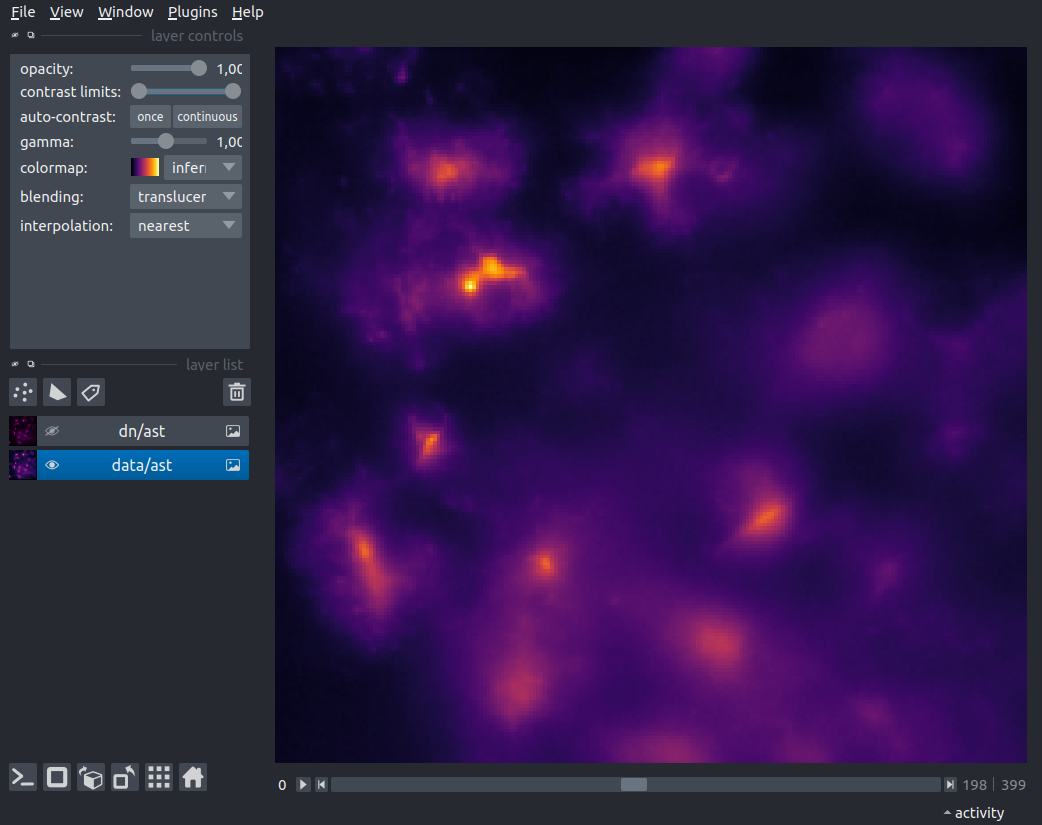
\includegraphics[width=\linewidth]{figures/2.png}
\end{center}
\caption{Screenshot of the \ac{GUI} displaying the converted video file of astrocytic calcium fluorescence (\ref{Tbl1}). The video has been downsampled and captured at a 20X magnification, focusing on the \ac{preBötC} region.}\label{fig:2}
\end{figure}

\begin{figure}[h!]
\begin{center}
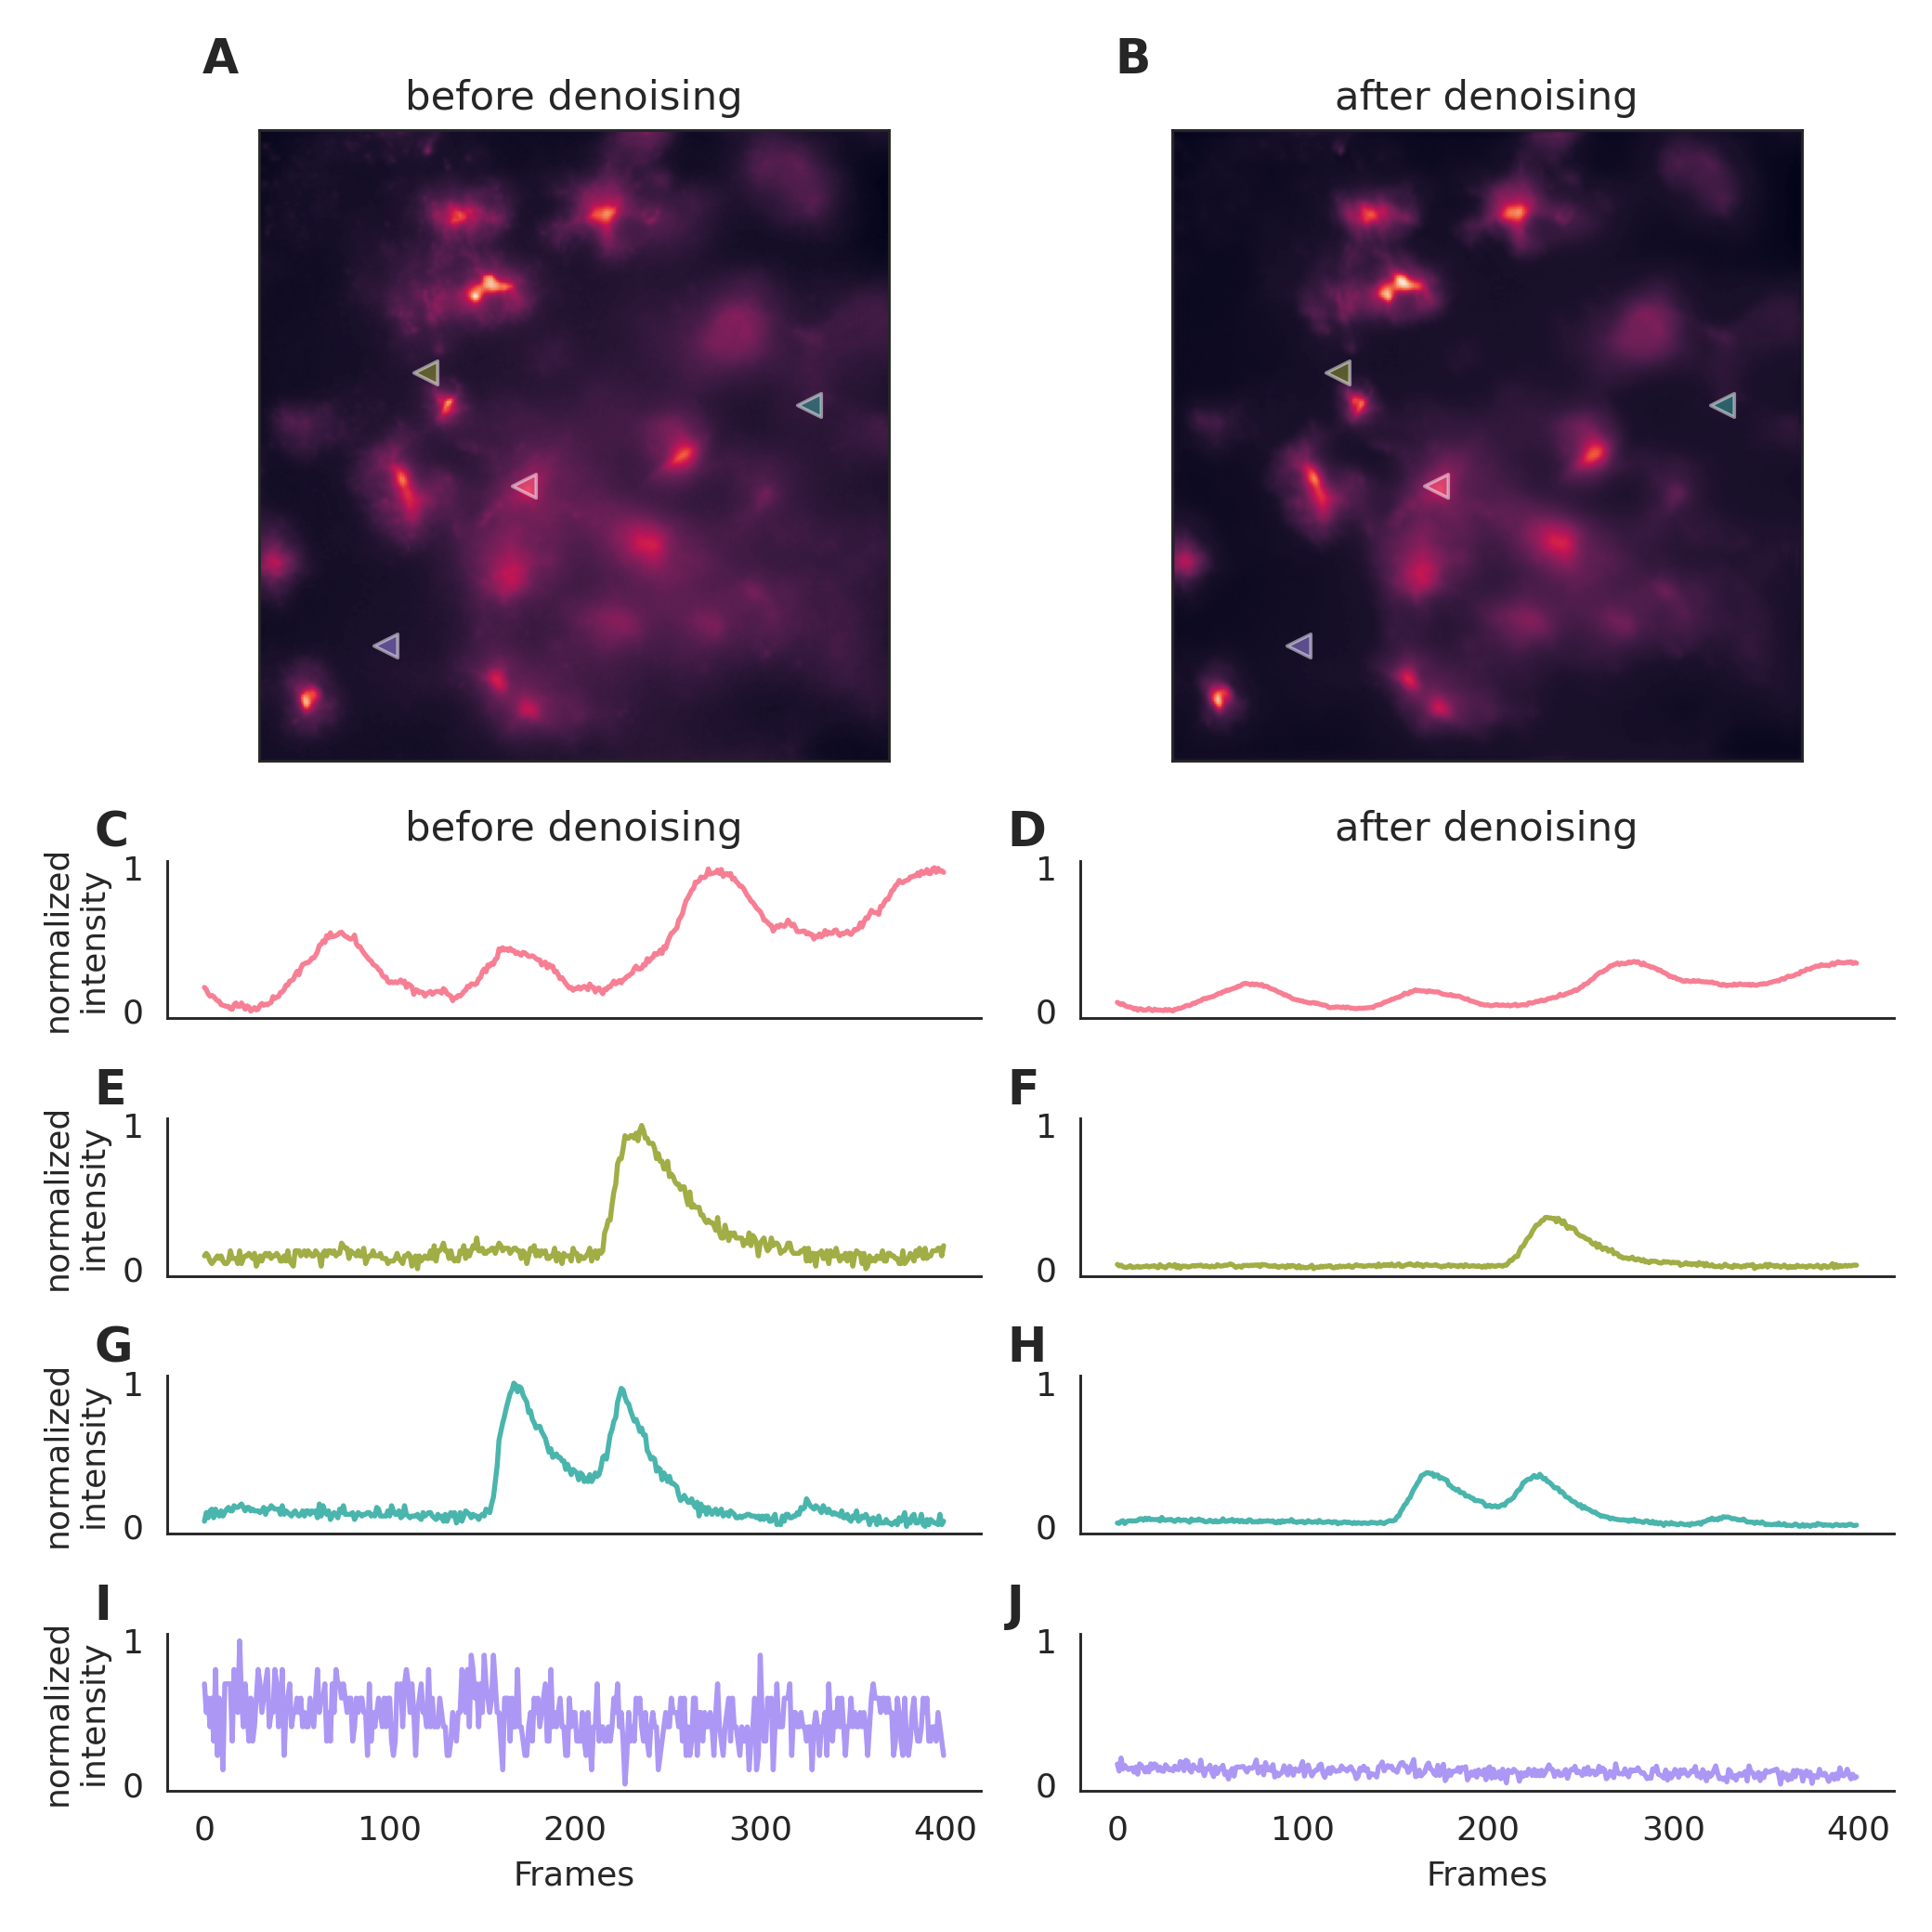
\includegraphics[width=\linewidth]{figures/3.png}
\end{center}
\caption{Comparative Visualization of Denoising on Video Frames and Pixel Intensity Measurements. Single frame (512x512 pixels) before denoising (left panel), showing notable background, and the corresponding frame after the application of a denoising algorithm, showing reduced background and enhanced clarity (middle panel). Pixel intensity traces from four selected points (right panel, P0-P3) in the video frame before denoising, displaying the variation over 200 frames. Right Plot) Pixel intensity traces for the same points after denoising, indicating a more stable intensity profile, while retaining features of the signal. The denoising algorithm was applied to a (128, 128) field of view with a configuration of 5 frames, each bordering the target frame, and no gap frames. The denoiser, trained for 50 epochs on a custom dataset, had a learning rate of 0.0001, momentum of 0.9, 3 layer stacks (n\_stacks), and 64 kernels of size 3 in the first layer without batch normalization. Inference involved a 10-pixel overlap in each direction with 'edge' padding. The test and validation were conducted using the same custom training dataset.
}\label{fig:3}
\end{figure}

\begin{figure}[h!]
\begin{center}
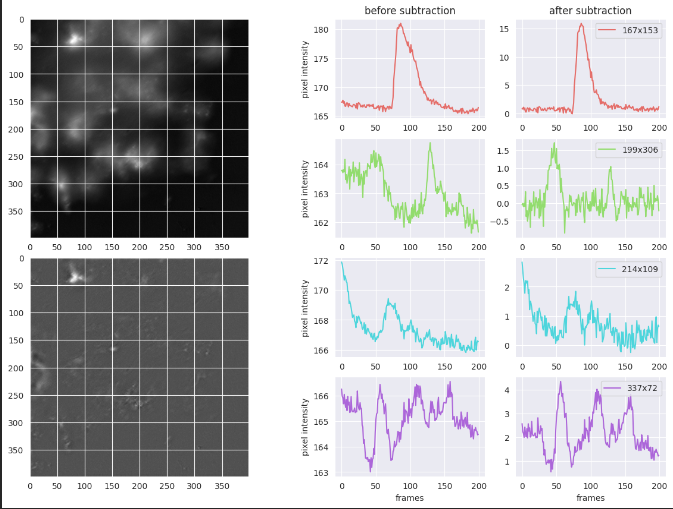
\includegraphics[width=\linewidth]{figures/4.png}
\end{center}
\caption{Background Subtraction in Fluorescence Imaging Analysis. Comparative analysis of fluorescence images and pixel intensity traces before (top left) and after background subtraction (bottom left). Pixel intensity over time (right panels). These plots reveal the background noise reduction, where post-subtraction y-axis values are near zero, indicating effective subtraction. Event shapes remain consistent, verifying reliable preservation of events. Notably, the second panel (green) slightly alters the signal strength of events, underscoring the importance of careful parameter optimization or exclusion of this step if it compromises data fidelity. Please refer to Video S2\ref{} for a dynamic visualization.}\label{fig:4}
\end{figure}

\begin{figure}[h!]
\begin{center}
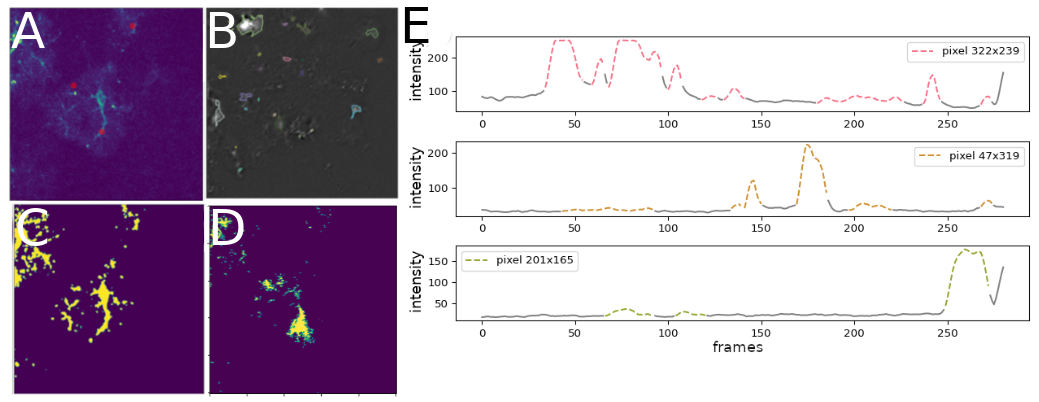
\includegraphics[width=\linewidth]{figures/5.png}
\end{center}
\caption{Overview of Event Detection in Calcium Fluorescence Imaging. A) Calcium Fluorescence Processing: Post-motion correction and denoising, showcasing calcium fluorescence. Red dots signify the selected pixels for detailed analysis in Panel E. B) Event Identification: Events detected through both temporal and spatial thresholding techniques. Colored regions highlight the active events within specific pixels, illustrating the spatial distribution of neuronal activity. C) Temporal Thresholding: A binary mask generated by applying a temporal threshold, delineating periods of significant activity versus inactivity. D) Spatial Thresholding: A binary mask created by spatial thresholding to identify active regions, emphasizing the spatial aspects of neuronal activity. E) Pixel Intensity Analysis: Examination of pixel intensities for pixels indicated in Panel A. Colored regions within the plot correspond to frames identified as active, providing a temporal resolution of neuronal activity.}\label{fig:5}
\end{figure}




\end{document}

%\section{Level1}
%\subsection{Level 2}
%\subsubsection{Level 3}
%\paragraph{Level 4}
%\subparagraph{Level 5}
